\documentclass[12pt]{article}
\usepackage[margin=1in]{geometry}
\usepackage{amsmath}
\usepackage{amssymb}
\usepackage{amsfonts}
\usepackage{amsthm}
\newtheorem{thm}{Theorem}[section]
\newtheorem{cor}[thm]{Corollary}
\newtheorem{lem}[thm]{Lemma}
\newtheorem{prop}[thm]{Proposition}
\usepackage{tikz-cd}
\renewcommand{\d}{\mathrm{d}}

\begin{document}

\title{Math 180 Homework 8}
\author{Nathan Solomon}
\maketitle

\section{}
\noindent\fbox{\fbox{\parbox{6.5in}{
            Consider a random graph $G$ on $3n$ vertices where each edge is chosen independently with probability $\frac{1}{2}$. Show that the probability that $G$ contains a triangle (i.e. $K_3$) goes to 1 as $n \rightarrow \infty$.
}}}\bigskip\par
Let $a$ be any vertex of $G$. Since there are $3n-1$ other vertices, the probability that the $ \operatorname{deg}(a) = y$ is $\binom{3n-1}{y}2^{1-3n}$.
If $a$ is connected to $y$ vertices, the chance that there is at least one edge in the subgraph made of those $y$ vertices is $1-( \frac{1}{2})^{\binom{y}{2}}$.
Therefore, the chance that $G$ contains a triangle which contains $a$ is
\[ \sum_{y=2}^{3n-1} \left( \binom{3n-1}{y} 2^{1-3n} \left( 1- \frac{1}{2^{y(y-1)/2}} \right)  \right), \]
and the chance that $G$ contains a triangle is even higher. We can evaluate the limit of that sum as $n \rightarrow \infty$ by noting that if we ignore the terms for which $y << n$, then the sum becomes
\[ \sum_{y > \varepsilon n}^{3n-1} \left( 2^{1-3n} \binom{3n-1}{y} \cdot 1 \right) \approx \sum_{y=0}^{3n-1} \left( 2^{1-3n} \binom{3n-1}{y} \right) = 1. \]
\par
\textit{Alternate method: show that if $G$ has $n>2$ vertices and at least $n^2/4$ edges, then it must contain a triangle, and the probability it has at least $n^2/4$ edges approaches 1 as $n \rightarrow \infty$.}

\section{}
\noindent\fbox{\fbox{\parbox{6.5in}{
            \textbf{Section 10.3, Problem 7.} (Markov inequality) Let $X$ be a random variable on some probability space attaining nonnegative values only. Let $\mu = \mathbb{E}[X]$ be its expectation, and let $t \geq 1$ be a real number. Prove that the probability that $X$ attains a value $\geq t\mu$ is at most $\frac{1}{t}$; in symbols,
            \[ P \left( \left\{ \omega \in \Omega : X(\omega) \geq t\mu \right\} \right) \leq \frac{1}{t}. \]
            (This is a simple but quite important inequality. It is often used if we want to show that the probability of some quantity getting too big is small.)
}}}\bigskip\par
\textit{Assume that $(\Omega, P)$ is a finite probability space. If it's not, we can just replace the sum here with an integral.}
\begin{align*}
    \mu = \mathbb{E}[X] &= \sum_{\omega \in \Omega} X(\omega)P(\omega) \\
                        &= \left( \sum_{\omega \in \Omega, X(\omega) \geq t\mu} X(\omega)P(\omega) \right) + \left( \sum_{\omega \in \Omega, X(\omega) < t\mu} X(\omega)P(\omega) \right) \\
\end{align*}
The first term in parentheses must be at least $t \mu P(X(\omega)\geq t\mu)$ and the second term in parentheses is nonnegative, so
\[ \mu \leq t \mu P \left( \left\{ \omega \in \Omega : X(\omega) \geq t\mu \right\} \right) \leq \frac{1}{t} \]
which means
\[ P \left( \left\{ \omega \in \Omega : X(\omega) \geq t\mu \right\} \right) \leq \frac{1}{t}. \]

\section{}
\noindent\fbox{\fbox{\parbox{6.5in}{
            \textbf{Section 10.3, Problem 8(a).}What is the expected number of surviving rabbits in Example 10.3.3 if there are $m$ rabbits and $n$ hunters?
            \begin{center}
                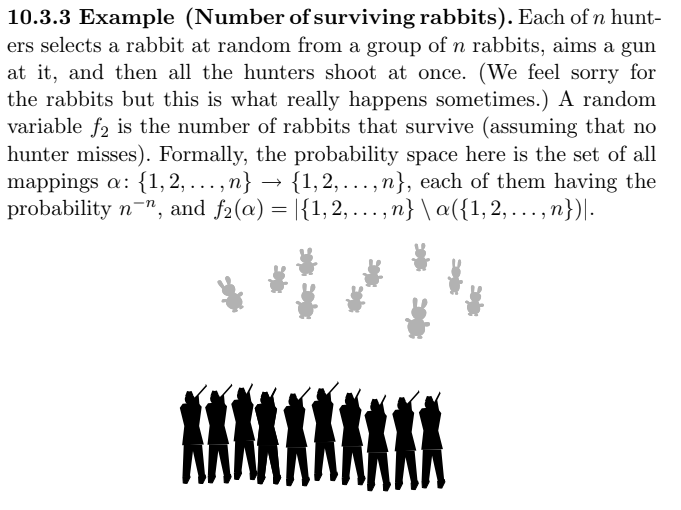
\includegraphics[width=\textwidth]{bunnies.png}
            \end{center}
}}}\bigskip\par
Each rabbit has a $\frac{1}{m}$ chance of being aimed at by each of the $n$ numters. Since every hunter aims independently, the chance of a rabbit being aimed at by no hunter is
\[ \left( 1- \frac{1}{m} \right)^n \]
so the expected number of rabbits that survives is approximately
\[ m \cdot \left( 1- \frac{1}{m} \right)^n. \]

\section{}
\noindent\fbox{\fbox{\parbox{6.5in}{
            Given a graph $G=(V,E)$, the MAXCUT problem is the problem of finding a partition of the vertices into disjoint subsets $A, B$ such that the number of edges with one endpoint in $A$ and other endpoint in $B$ is maximized. Show that there is a choice of $A,B$ with at least half the edges of $G$ going between them as follows.
            \begin{enumerate}
                \item Choose a random subset $A$ of $V$. You can do this in many ways, but it is easier if you do it in a way that maximizes independence.
                \item For each edge $e$, consider the indicator random variable for the event that $e$ has an endpoint in each part. Use linearity of expectation to compute the expected number of edges between $A$ and $B$.
                \item Use the pigeonhole principle for expectation and the probabilistic method.
            \end{enumerate}
}}}\bigskip\par
\begin{enumerate}
    \item Let $A$ be a random subset $A \subset V$ such that $|A|=|V|/2$ (or $|A|=(|V|-1)/2$, if $|V|$ is odd). Let $B=V \backslash A$.
    \item Let $f: E \rightarrow \left\{ 0,1 \right\}$ be the function such that $f(e)=1$ if and only if $e$ connects a vertex in $A$ to a vertex in $B$. The probability of $f$ being 1 is $\mathbb{E}(f)= \frac{1}{2}$. \textit{This is not quite true if $|V|$ is odd, but we can dumb this down by pretending $|V|$ is even, so the expected value of $f$ is one half. In reality, that probability is $\frac{2 \dot |A|\cdot|B|}{|V|^2}$, which could be a tiny bit less than one half. Part (3) of this proof would still work, but it would be a lot more painful.} By linearity of expectation, the expected number of edges between $A$ and $B$ is $\frac{|E|}{2}$.
    \item Either every choice of $A$ gives exactly $\frac{|E|}{2}$ edges between $A$ and $B$, or there are some choices of $A$ for which the number of edges between $A$ and $B$ is less than $\frac{|E|}{2}$ and some choices of $A$ for which it is more.
\end{enumerate}


\end{document}
